\documentclass[10pt]{beamer}
\usepackage[english]{babel}
\usepackage[utf8]{inputenc}
\usepackage[T1]{fontenc}
\usepackage{helvet}
\usepackage{ragged2e}
%-------------------------------------------------------
% INFORMATION IN THE TITLE PAGE
%-------------------------------------------------------

\newcommand{\cstitle}{\textbf{Bioinformatics}}
\subtitle[]{Neighbor Joining}
\newcommand{\cscourseCode}{1005155}
\newcommand{\csauthor}{MSc. Vicente Machaca Arceda}
\institute[UNSA]{Universidad Nacional de San Agustín de Arequipa}
\newcommand{\csemail}{vmachacaa@unsa.edu.pe}
\newcommand{\instituteabr}{UNSA}
\newcommand{\nameUp}{ICC Fase 1}
\date{\today}
\title[\cscourseCode]{\cstitle}
\author{\csauthor}
%%%%%%%%%%%%%%%%%

%-------------------------------------------------------
% SOLUTION
%-------------------------------------------------------
\def\mysol{0} 
\def\mysol{1} 
%-------------------------------------------------------


%-------------------------------------------------------
% CHOOSE THE THEME
%-------------------------------------------------------
\def\mycmd{0} % CS THEME
%\def\mycmd{1} % MYTHEME
%-------------------------------------------------------


\if\mycmd1
\usetheme[]{Feather}
\newcommand{\chref}[2]{	\href{#1}{{\usebeamercolor[bg]{Feather}#2}} }
\else
\usepackage{csformat}
\fi

\newcommand{\1}{
	\setbeamertemplate{background}{
		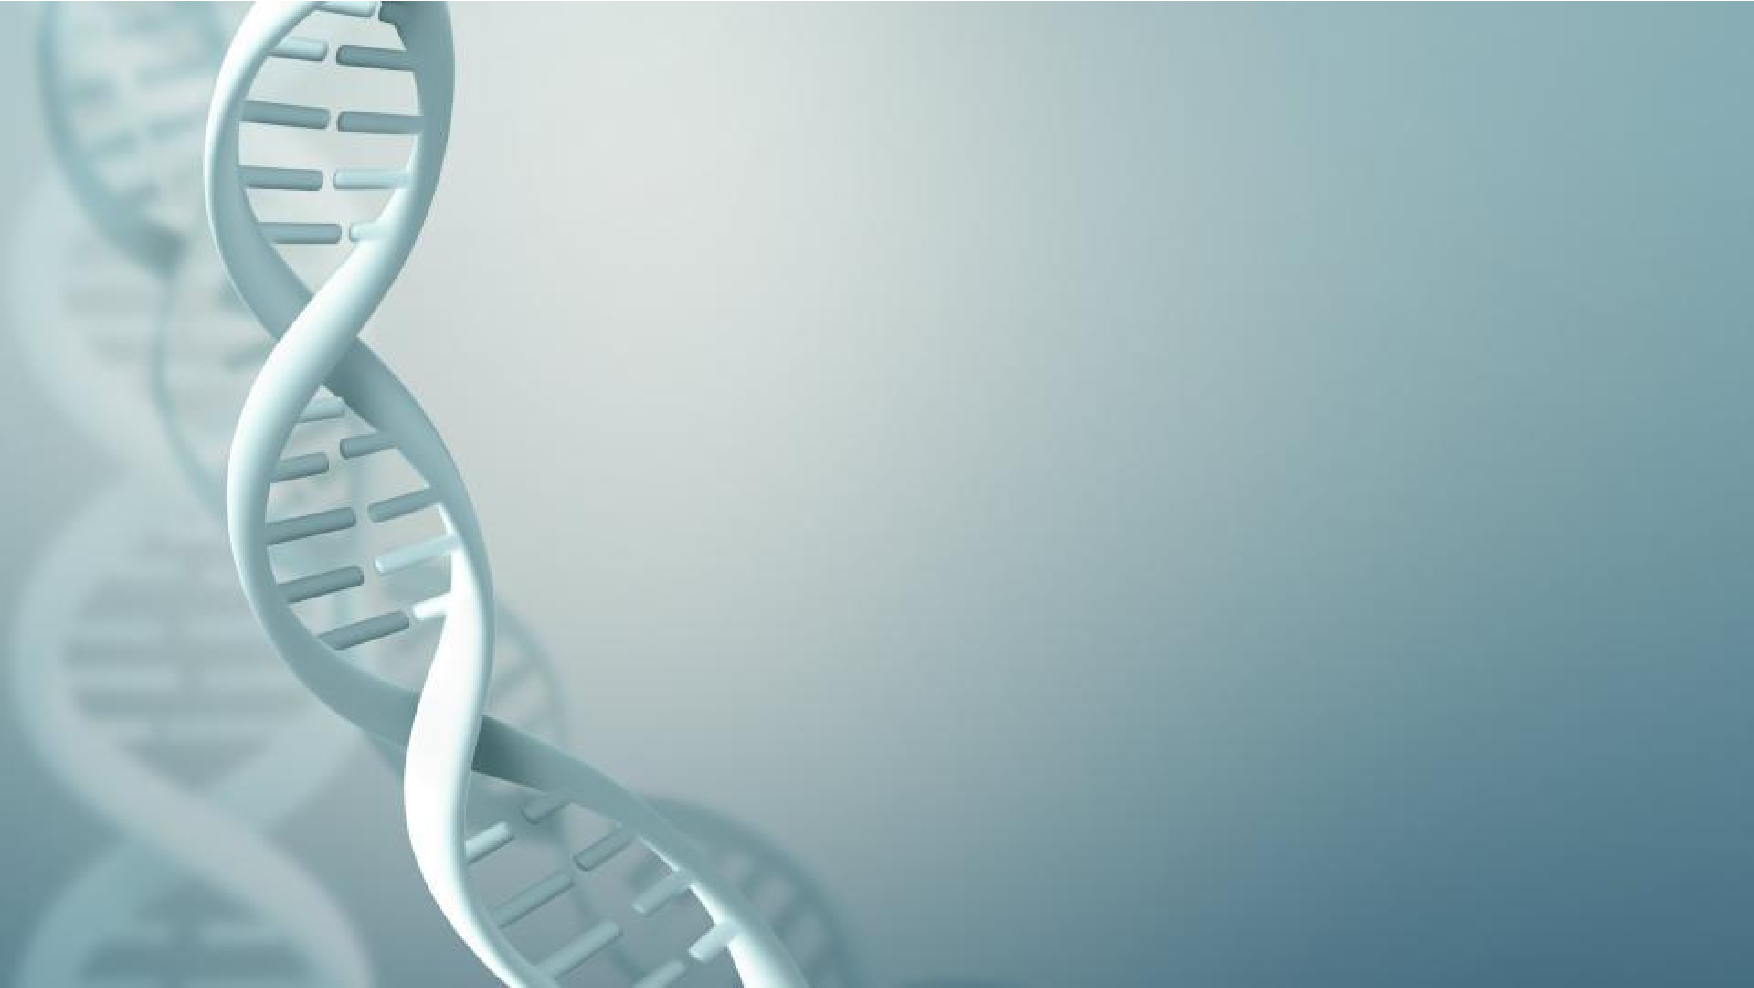
\includegraphics[width=\paperwidth,height=\paperheight]{img/1}
		\tikz[overlay] \fill[fill opacity=0.75,fill=white] (0,0) rectangle (-\paperwidth,\paperheight);
	}
}



%-------------------------------------------------------
% THE BODY OF THE PRESENTATION
%-------------------------------------------------------

\begin{document}
	
	
	\AtBeginSubsection[]
	{
		\begin{frame}
			\frametitle{Table of Contents}
			\tableofcontents[currentsubsection]
		\end{frame}
	}
	
	
	%-------------------------------------------------------
	% THE TITLEPAGE
	%-------------------------------------------------------
	
	\if\mycmd1 % MY THEME
	\1{
		\begin{frame}[plain,noframenumbering] 
			\titlepage 
		\end{frame}}
		\else % CS THEME
		\maketitle
		\fi

%-------------------------------------------------------
%-------------------------------------------------------
\begin{frame}{Table of Contents}
\tableofcontents
\end{frame}
%-------------------------------------------------------
%-------------------------------------------------------

%%%%%%%%%%%%%%%%%%%%%%%%%%%%%%%%%%%%%%%%%%%%%%%%%%%%%%%%%%%%%%%%%%%%%%%%%%%%%%%%%%%%%%%%%%%%%%%%%%%%%%%%%%%%%%%%
%%%%%%%%%%%%%%%%%%%%%%%%%%%%%%%%%%%%%%%%%%%%%%%%%%%%%%%%%%%%%%%%%%%%%%%%%%%%%%%%%%%%%%%%%%%%%%%%%%%%%%%%%%%%%%%%
\section{Introduction}
%%%%%%%%%%%%%%%%%%%%%%%%%%%%%%%%%%%%%%%%%%%%%%%%%%%%%%%%%%%%%%%%%%%%%%%%%%%%%%%%%%%%%%%%%%%%%%%%%%%%%%%%%%%%%%%%
%%%%%%%%%%%%%%%%%%%%%%%%%%%%%%%%%%%%%%%%%%%%%%%%%%%%%%%%%%%%%%%%%%%%%%%%%%%%%%%%%%%%%%%%%%%%%%%%%%%%%%%%%%%%%%%%

%%%%%%%%%%%%%%%%%%%%%%%%%%%%%%%%%%%%%%%%%%%%%%%%%%%%%%%%%%%%%%%%%%%%%%%%%%%%%%%%%%%%%%%%%%%%%%%%%%%%%%%%%%%%%%%%
%%%%%%%%%%%%%%%%%%%%%%%%%%%%%%%%%%%%%%%%%%%%%%%%%%%%%%%%%%%%%%%%%%%%%%%%%%%%%%%%%%%%%%%%%%%%%%%%%%%%%%%%%%%%%%%%
\subsection{Objectives}
%%%%%%%%%%%%%%%%%%%%%%%%%%%%%%%%%%%%%%%%%%%%%%%%%%%%%%%%%%%%%%%%%%%%%%%%%%%%%%%%%%%%%%%%%%%%%%%%%%%%%%%%%%%%%%%%
%%%%%%%%%%%%%%%%%%%%%%%%%%%%%%%%%%%%%%%%%%%%%%%%%%%%%%%%%%%%%%%%%%%%%%%%%%%%%%%%%%%%%%%%%%%%%%%%%%%%%%%%%%%%%%%%

%-------------------------------------------------------
%-------------------------------------------------------
\begin{frame}{Introduction}{Objectives}
\begin{itemize} 
    \item<1-> Understand and implement Neighbor joining algorithm to biild phylogenetics trees.
  \end{itemize}
\end{frame}
%-------------------------------------------------------
%-------------------------------------------------------


%%%%%%%%%%%%%%%%%%%%%%%%%%%%%%%%%%%%%%%%%%%%%%%%%%%%%%%%%%%%%%%%%%%%%%%%%%%%%%%%%%%%%%%%%%%%%%%%%%%%%%%%%%%%%%%%
%%%%%%%%%%%%%%%%%%%%%%%%%%%%%%%%%%%%%%%%%%%%%%%%%%%%%%%%%%%%%%%%%%%%%%%%%%%%%%%%%%%%%%%%%%%%%%%%%%%%%%%%%%%%%%%%
\subsection{Methods}
%%%%%%%%%%%%%%%%%%%%%%%%%%%%%%%%%%%%%%%%%%%%%%%%%%%%%%%%%%%%%%%%%%%%%%%%%%%%%%%%%%%%%%%%%%%%%%%%%%%%%%%%%%%%%%%%
%%%%%%%%%%%%%%%%%%%%%%%%%%%%%%%%%%%%%%%%%%%%%%%%%%%%%%%%%%%%%%%%%%%%%%%%%%%%%%%%%%%%%%%%%%%%%%%%%%%%%%%%%%%%%%%%

%-------------------------------------------------------
%-------------------------------------------------------
\begin{frame}{Phylogenetics}{Methods}
	\begin{figure}
		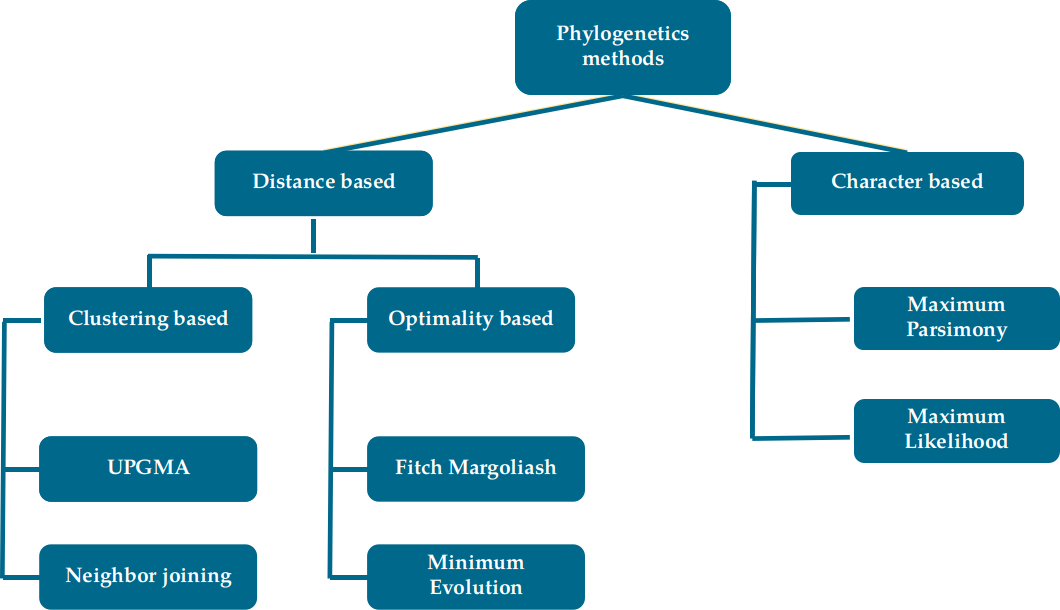
\includegraphics[width=\textwidth]{img/philo/methods}
		\caption{The most used methods to build philogenetic trees.}			
	\end{figure}
\end{frame}
%-------------------------------------------------------
%-------------------------------------------------------

%%%%%%%%%%%%%%%%%%%%%%%%%%%%%%%%%%%%%%%%%%%%%%%%%%%%%%%%%%%%%%%%%%%%%%%%%%%%%%%%%%%%%%%%%%%%%%%%%%%%%%%%%%%%%%%%
%%%%%%%%%%%%%%%%%%%%%%%%%%%%%%%%%%%%%%%%%%%%%%%%%%%%%%%%%%%%%%%%%%%%%%%%%%%%%%%%%%%%%%%%%%%%%%%%%%%%%%%%%%%%%%%%
\section{Neighbor joining}
%%%%%%%%%%%%%%%%%%%%%%%%%%%%%%%%%%%%%%%%%%%%%%%%%%%%%%%%%%%%%%%%%%%%%%%%%%%%%%%%%%%%%%%%%%%%%%%%%%%%%%%%%%%%%%%%
%%%%%%%%%%%%%%%%%%%%%%%%%%%%%%%%%%%%%%%%%%%%%%%%%%%%%%%%%%%%%%%%%%%%%%%%%%%%%%%%%%%%%%%%%%%%%%%%%%%%%%%%%%%%%%%%

%%%%%%%%%%%%%%%%%%%%%%%%%%%%%%%%%%%%%%%%%%%%%%%%%%%%%%%%%%%%%%%%%%%%%%%%%%%%%%%%%%%%%%%%%%%%%%%%%%%%%%%%%%%%%%%%
%%%%%%%%%%%%%%%%%%%%%%%%%%%%%%%%%%%%%%%%%%%%%%%%%%%%%%%%%%%%%%%%%%%%%%%%%%%%%%%%%%%%%%%%%%%%%%%%%%%%%%%%%%%%%%%%
\subsection{Method}
%%%%%%%%%%%%%%%%%%%%%%%%%%%%%%%%%%%%%%%%%%%%%%%%%%%%%%%%%%%%%%%%%%%%%%%%%%%%%%%%%%%%%%%%%%%%%%%%%%%%%%%%%%%%%%%%
%%%%%%%%%%%%%%%%%%%%%%%%%%%%%%%%%%%%%%%%%%%%%%%%%%%%%%%%%%%%%%%%%%%%%%%%%%%%%%%%%%%%%%%%%%%%%%%%%%%%%%%%%%%%%%%%

%-------------------------------------------------------
%-------------------------------------------------------
\begin{frame}{Neighbor joining}{Definition}
	\begin{block}{}
		The UPGMA method uses unweighted distances and assumes that all taxa have constant evolutionary rates.
	\end{block}
	
	\begin{block}{}
		Neighbor joining (NJ) does not assume the taxa to be equidistant from the root. It corrects for unequal
		evolutionary rates between sequences by using a conversion step.
	\end{block}
\end{frame}
%-------------------------------------------------------
%-------------------------------------------------------

%-------------------------------------------------------
%-------------------------------------------------------
\begin{frame}{Neighbor joining}{Definition}
NJ requires the calculations of “r-values” and “transformed r-values” using:

\begin{equation}\label{eq:nj_1}
	d'_{AB} = d_{AB} - \frac{1}{2}(r_A + r_B)
\end{equation} 

\begin{itemize}
	\item $d'_{AB}$ is the converted distance between $A$ and $B$.
	\item $d_{AB}$ is the actual evolutionary distance between $A$ and $B$.
	\item $r_A$ (or $r_B$) is the sum of distances of $A$ (or $B$)
	to all other taxa.
\end{itemize}	
\end{frame}
%-------------------------------------------------------
%-------------------------------------------------------


%-------------------------------------------------------
%-------------------------------------------------------
\begin{frame}{Neighbor joining}{Definition}
	The r-values are needed to create a modified
	distance matrix:
		
	\begin{equation}\label{eq:nj_2}
		r_i = \sum d_{ij}
	\end{equation} 
	
	\begin{itemize}
		\item $i$ and $j$ are two different taxa.
	\end{itemize}	

	\vspace{0.5cm}
	
	The transformed r-values ($r'$ ) are used to determine the distances of
	an individual taxon to the nearest node:
	
	\begin{equation}\label{eq:nj_3}
	r'_i =  \frac{r_i}{n-2}
	\end{equation} 
	\begin{itemize}
		\item $n$ is the total number of taxa.
	\end{itemize}
\end{frame}
%-------------------------------------------------------
%-------------------------------------------------------

%-------------------------------------------------------
%-------------------------------------------------------
\begin{frame}{Neighbor joining}{Definition}
	Assuming $A$ and $B$ form a node called
	$U$, the distance $A$ to $U$ is determined by the following formula:
	
	\begin{equation}\label{eq:nj_4}
		d_{AU} = \frac{ d_{AB} + ( r'_A - r'_B ) }{2}
	\end{equation} 
	
\end{frame}
%-------------------------------------------------------
%-------------------------------------------------------


%%%%%%%%%%%%%%%%%%%%%%%%%%%%%%%%%%%%%%%%%%%%%%%%%%%%%%%%%%%%%%%%%%%%%%%%%%%%%%%%%%%%%%%%%%%%%%%%%%%%%%%%%%%%%%%%
%%%%%%%%%%%%%%%%%%%%%%%%%%%%%%%%%%%%%%%%%%%%%%%%%%%%%%%%%%%%%%%%%%%%%%%%%%%%%%%%%%%%%%%%%%%%%%%%%%%%%%%%%%%%%%%%
\subsection{Example}
%%%%%%%%%%%%%%%%%%%%%%%%%%%%%%%%%%%%%%%%%%%%%%%%%%%%%%%%%%%%%%%%%%%%%%%%%%%%%%%%%%%%%%%%%%%%%%%%%%%%%%%%%%%%%%%%
%%%%%%%%%%%%%%%%%%%%%%%%%%%%%%%%%%%%%%%%%%%%%%%%%%%%%%%%%%%%%%%%%%%%%%%%%%%%%%%%%%%%%%%%%%%%%%%%%%%%%%%%%%%%%%%%

%-------------------------------------------------------
%-------------------------------------------------------
\begin{frame}{Neighbor joining}{Example}
	\begin{columns}
		\begin{column}{0.48\textwidth}
			\begin{figure}
				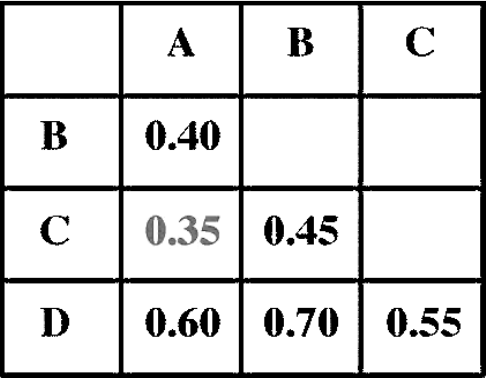
\includegraphics[width=\textwidth]{img/philo/NJ_1}
				%\caption{Image example in 2 gray levels.}
			\end{figure}
		\end{column}
		\begin{column}{0.48\textwidth}
			The first step of the NJ method is $r$-value and $r'$-value calculation. According to Eq. \ref{eq:nj_2} and \ref{eq:nj_3}.			
		\end{column}
	\end{columns}
\end{frame}
%-------------------------------------------------------
%-------------------------------------------------------



%-------------------------------------------------------
%-------------------------------------------------------
\begin{frame}{Neighbor joining}{Example}
	\begin{columns}
		\begin{column}{0.48\textwidth}
			\begin{figure}
				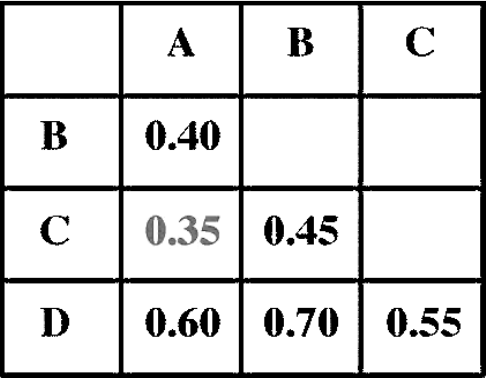
\includegraphics[width=\textwidth]{img/philo/NJ_1}
				%\caption{Image example in 2 gray levels.}
			\end{figure}
		\end{column}
		\begin{column}{0.48\textwidth}
			Eq. \ref{eq:nj_2} and \ref{eq:nj_3}.	
			\begin{equation*}
				r_i = \sum d_{ij}; r'_i =  \frac{r_i}{n-2}
			\end{equation*} 
			
			For node $A$:
			\begin{equation*}
			r_A = d_{AB} + d_{AC} + d_{AD} = 0.4 + 0.35 + 0.6
			\end{equation*}
			\begin{equation*}
			r_A  = 1.35
			\end{equation*}
			
			\begin{equation*}
			r'_A =  \frac{1.35}{4-2}
			\end{equation*}  
		\end{column}
	\end{columns}
\end{frame}
%-------------------------------------------------------
%-------------------------------------------------------

%-------------------------------------------------------
%-------------------------------------------------------
\begin{frame}{Neighbor joining}{Example}
	\begin{columns}
		\begin{column}{0.48\textwidth}
			\begin{figure}
				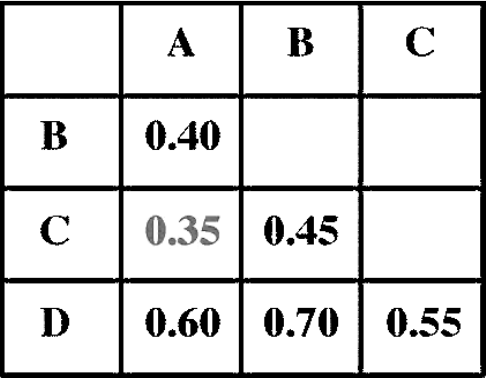
\includegraphics[width=\textwidth]{img/philo/NJ_1}
				%\caption{Image example in 2 gray levels.}
			\end{figure}
		\end{column}
		\begin{column}{0.48\textwidth}
			Eq. \ref{eq:nj_2} and \ref{eq:nj_3}.	
			\begin{equation*}
			r_i = \sum d_{ij}; r'_i =  \frac{r_i}{n-2}
			\end{equation*} 
			
			Do the same for nodes $B, C$ and $D$:
		\end{column}
	\end{columns}
\end{frame}
%-------------------------------------------------------
%-------------------------------------------------------

%-------------------------------------------------------
%-------------------------------------------------------
\if\mysol1
\begin{frame}{Neighbor joining}{Example}
	\begin{columns}
		\begin{column}{0.48\textwidth}
			\begin{figure}
				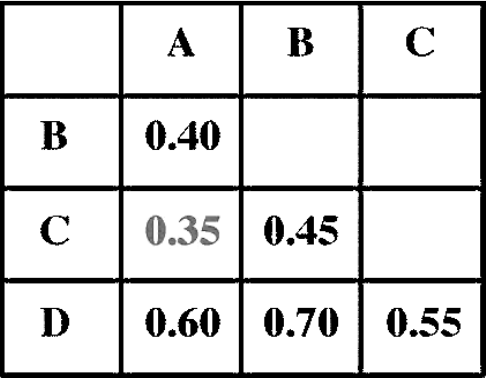
\includegraphics[width=\textwidth]{img/philo/NJ_1}
				%\caption{Image example in 2 gray levels.}
			\end{figure}
		\end{column}
		\begin{column}{0.48\textwidth}
			\begin{equation*}
				\begin{split}
					r_A = 1.35 ; r'_A = 0.675  \\
					r_B = 1.55 ; r'_B = 0.775 \\ 
					r_C = 1.35 ; r'_C = 0.675 \\ 
					r_D = 1.85 ; r'_D = 0.925 
				\end{split}
			\end{equation*} 
			
			
		\end{column}
	\end{columns}
\end{frame}
\fi
%-------------------------------------------------------
%-------------------------------------------------------

%-------------------------------------------------------
%-------------------------------------------------------
\begin{frame}{Neighbor joining}{Example}
	\begin{columns}
		\begin{column}{0.48\textwidth}
			\begin{figure}
				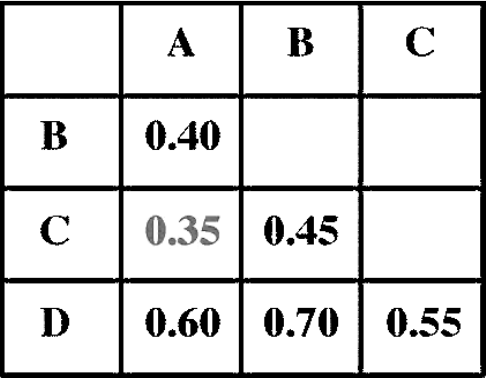
\includegraphics[width=\textwidth]{img/philo/NJ_1}
				%\caption{Image example in 2 gray levels.}
			\end{figure}
		\end{column}
		\begin{column}{0.48\textwidth}
			Calculate $d'_{ij}$ using Eq. \ref{eq:nj_1}.	
			\begin{equation*}
				d'_{AB} = d_{AB} - \frac{1}{2}(r_A + r_B)
			\end{equation*} 
			
		\end{column}
	\end{columns}
\end{frame}
%-------------------------------------------------------
%-------------------------------------------------------

%-------------------------------------------------------
%-------------------------------------------------------
\if\mysol1
\begin{frame}{Neighbor joining}{Example}
	\begin{columns}
		\begin{column}{0.48\textwidth}
			\begin{figure}
				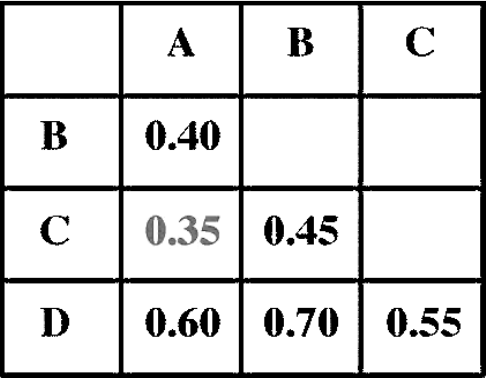
\includegraphics[width=\textwidth]{img/philo/NJ_1}
				%\caption{Image example in 2 gray levels.}
			\end{figure}
		\end{column}
		\begin{column}{0.48\textwidth}
			\begin{equation*}
			\begin{split}
				d'_{AB} = -1.05 \\
				d'_{AC} = -1.00 \\
				d'_{AD} = -1.00 \\
				d'_{BC} = -1.00 \\
				d'_{BD} = -1.00 \\
				d'_{CD} = -1.05 \\
			\end{split}
			\end{equation*} 			
		\end{column}
	\end{columns}
\end{frame}
\fi
%-------------------------------------------------------
%-------------------------------------------------------

%-------------------------------------------------------
%-------------------------------------------------------
\begin{frame}{Neighbor joining}{Example}
	\begin{columns}
		\begin{column}{0.48\textwidth}
			The old distance matrix.
			\begin{figure}
				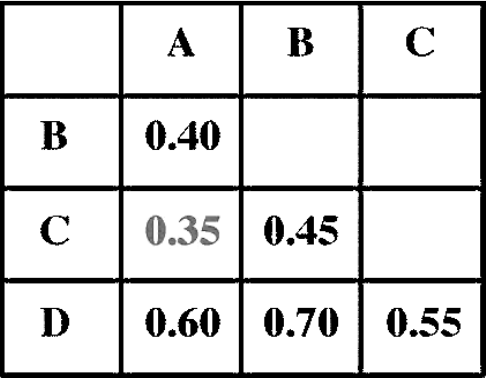
\includegraphics[width=\textwidth]{img/philo/NJ_1}
				%\caption{Image example in 2 gray levels.}
			\end{figure}
		\end{column}
		\begin{column}{0.48\textwidth}
			The new distance matrix.
			\begin{figure}
				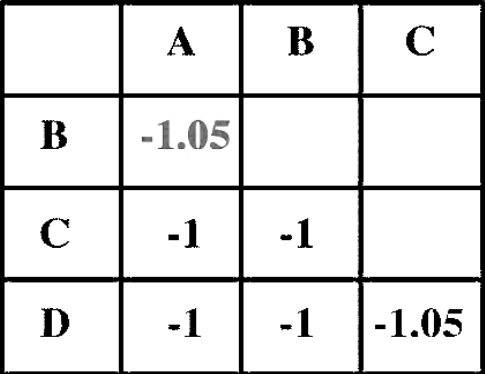
\includegraphics[width=\textwidth]{img/philo/NJ_2}
				%\caption{Image example in 2 gray levels.}
			\end{figure}		
		\end{column}
	\end{columns}
\end{frame}
%-------------------------------------------------------
%-------------------------------------------------------

%-------------------------------------------------------
%-------------------------------------------------------
\begin{frame}{Neighbor joining}{Example}

	The pair of taxa with the shortest distances in the new matrix are separated (either $AB$ or $CD$).
	
	\begin{figure}
		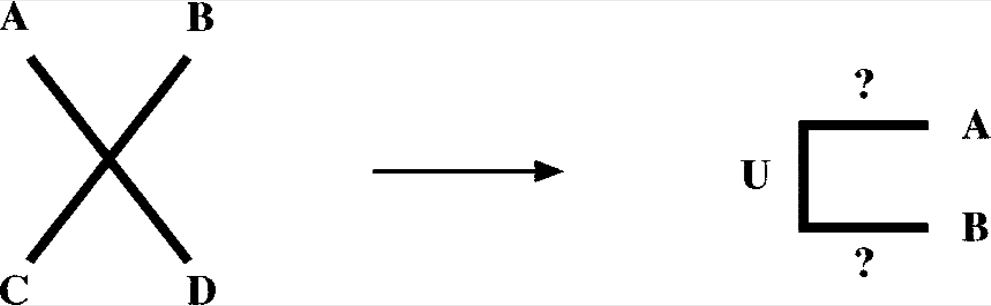
\includegraphics[width=\textwidth]{img/philo/NJ_3}
		%\caption{Image example in 2 gray levels.}
	\end{figure}

	Then, use Eq. \ref{eq:nj_4} to calculate $d_{AU}$ and $d_{BU}$.
	
\end{frame}
%-------------------------------------------------------
%-------------------------------------------------------

%-------------------------------------------------------
%-------------------------------------------------------
\begin{frame}{Neighbor joining}{Example}
	\begin{columns}
		\begin{column}{0.48\textwidth}
			\begin{figure}
				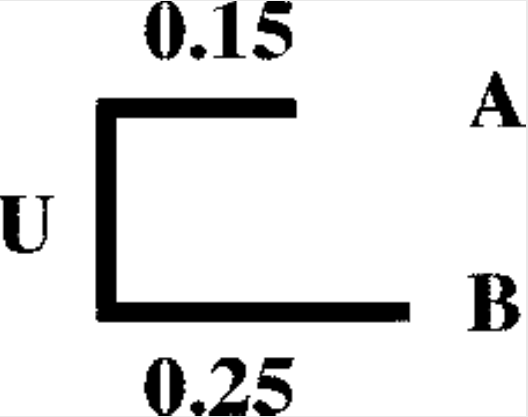
\includegraphics[width=0.6\textwidth]{img/philo/NJ_4}
				%\caption{Image example in 2 gray levels.}
			\end{figure}
		\end{column}
		\begin{column}{0.48\textwidth}
			Eq. \ref{eq:nj_4}:
			\begin{equation*}
				\begin{split}				
					d_{AU} = \frac{ d_{AB} + ( r'_A - r'_B ) }{2} = 0.15 \\
					d_{BU} = \frac{ d_{AB} + ( r'_B - r'_A ) }{2} = 0.25 \\
				\end{split}
			\end{equation*} 	
		\end{column}
	\end{columns}
\end{frame}
%-------------------------------------------------------
%-------------------------------------------------------


%-------------------------------------------------------
%-------------------------------------------------------
\begin{frame}{Neighbor joining}{Example}
	\begin{columns}
		\begin{column}{0.48\textwidth}
			\begin{figure}
				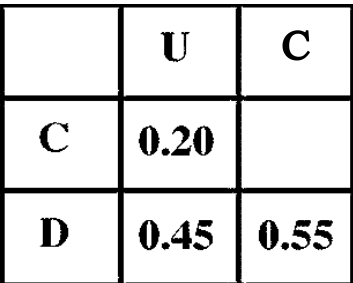
\includegraphics[width=0.7\textwidth]{img/philo/NJ_5}
				%\caption{Image example in 2 gray levels.}
			\end{figure}
		\end{column}
		\begin{column}{0.48\textwidth}
			Eq. \ref{eq:nj_4}:
			\begin{equation*}
			\begin{split}				
			d_{AU} = \frac{ d_{AB} + ( r'_A - r'_B ) }{2} = 0.15 \\
			d_{BU} = \frac{ d_{AB} + ( r'_B - r'_A ) }{2} = 0.25 \\
			\end{split}
			\end{equation*} 	
		\end{column}
	\end{columns}
\end{frame}
%-------------------------------------------------------
%-------------------------------------------------------


%-------------------------------------------------------
%-------------------------------------------------------
\if\mycmd1 % MY THEME
\1{
	{\1
		\begin{frame}[plain,noframenumbering]
			%\finalpage{Thank you}
			\begin{figure}[]
				\centering
				
\includegraphics[width=\textwidth,height=0.7\textheight,keepaspectratio]{img/question.png}
				%\label{img:mot2}
				%\caption{Image example in 2 gray levels.}
			\end{figure}
	\end{frame}}
	\else % CS THEME
	\begin{frame}{Questions?}
		\begin{figure}[]
			\centering
			
\includegraphics[width=\textwidth,height=0.7\textheight,keepaspectratio]{img/question.png}
			%\label{img:mot2}
			%\caption{Image example in 2 gray levels.}
		\end{figure}
		
	\end{frame}
	\fi
	%-------------------------------------------------------
	%-------------------------------------------------------

%-------------------------------------------------------
%-------------------------------------------------------
%\begin{frame}[allowframebreaks]
%	\frametitle{References}
	%\bibliographystyle{amsalpha}
%	\bibliographystyle{IEEEtran}
%	\bibliography{bibliography.bib}
%\end{frame}
%-------------------------------------------------------
%-------------------------------------------------------

\end{document}